\documentclass[10pt, a4paper,english,spanish]{article}
\usepackage{subfig}

\parindent=20pt
\parskip=8pt
\usepackage[width=15.5cm, left=3cm, top=2.5cm, height= 24.5cm]{geometry}

\usepackage{ccfonts,eulervm} 
\usepackage[T1]{fontenc}
\usepackage{epigraph}
\usepackage{amsmath}
\usepackage{amsfonts}
\usepackage{amssymb}
\usepackage{fancyhdr}
\usepackage[activeacute, spanish]{babel}
\usepackage{cancel}
\usepackage[utf8]{inputenc}
\usepackage{algorithm}
\usepackage{algpseudocode}
\usepackage{afterpage}
\usepackage{caratula}
\usepackage{url}
\usepackage{fancyhdr}

\floatname{algorithm}{Algoritmo}

\newtheorem{theorem}{Teorema}[section]
\newtheorem{lemma}[theorem]{Lema}
\newtheorem{proposition}[theorem]{Proposici\'on}
\newtheorem{corollary}[theorem]{Corolario}

\newcommand{\Var}{\textbf{var }}
\newcommand{\True}{\textbf{true }}
\newcommand{\False}{\textbf{false }}
\newcommand{\Break}{\textbf{break }}
\newcommand{\Continue}{\textbf{continue }}
\newcommand{\Param}{\textbf{param }}

\newenvironment{proof}[1][Demostraci\'on]{\begin{trivlist}
\item[\hskip \labelsep {\bfseries #1}]}{\end{trivlist}}
\newenvironment{definition}[1][Definici\'on]{\begin{trivlist}
\item[\hskip \labelsep {\bfseries #1}]}{\end{trivlist}}
\newenvironment{example}[1][Ejemplo]{\begin{trivlist}
\item[\hskip \labelsep {\bfseries #1}]}{\end{trivlist}}
\newenvironment{remark}[1][Observaci\'on]{\begin{trivlist}
\item[\hskip \labelsep {\bfseries #1}]}{\end{trivlist}}

\newcommand{\qed}{\nobreak \ifvmode \relax \else
      \ifdim\lastskip<1.5em \hskip-\lastskip
      \hskip1.5em plus0em minus0.5em \fi \nobreak
      \vrule height0.75em width0.5em depth0.25em\fi}

\parindent 0em
\algrenewcommand{\algorithmiccomment}[1]{//\textit{#1} }

\pagestyle{fancy}
\thispagestyle{fancy}
\addtolength{\headheight}{1pt}
\lhead{ORGA 2 - TP FINAL}
\rhead{Grupo 2}
\cfoot{\thepage}
\renewcommand{\footrulewidth}{0.4pt}
\newcommand{\hblacksquare}{\hfill \blacksquare}
%FIN COPYPASTE EL INFORME DEL INFO
\begin{document}

\materia{Organizaci\'on del Computador II - Trabajo Pr\'actico Final}
\submateria{Primer Cuatrim\'estre de 2012}
\titulo{Prototipo de Sistema Operativo}
\subtitulo{Informe}
\integrante{Juan Pablo Darago}{272/10}{jpdarago@gmail.com}

\maketitle
\pagebreak

\tableofcontents
\pagebreak

\section{Introducci\'on}

\epigraph{I'm doing a (free) operating system (just a hobby, won't be big and professional like gnu) for 386(486) AT clones.}{Linus Torvalds,
anunciando Linux por \url{news:comp.os.minix} }

El siguiente trabajo se presenta como complemento y documentaci\'on
del trabajo pr\'actico final realizado para la materia Organizaci\'on
del Computador II. 

El trabajo pr\'actico final fue realizado sobre el tema de programaci\'on
de sistemas operativos sobre la arquitectura Intel IA-32, correspondiente
a la segunda parte de la cursada de la materia en el segundo cuatrimestre
de 2011.

El prop\'osito de este informe es detallar las decisiones de dise\~no
y los problemas y soluciones encontrados durante la implementaci\'on del
prototipo de Sistema Operativo que se incluye con este informe.

\section{Alcance y prop\'osito del trabajo}

Se busc\'o implementar un Sistema Operativo monousuario y multitarea,
utilizando para ello las facilidades para el manejo de tareas en nivel de
usuario y dem\'as recursos que se hacen disponibles mediante la arquitectura
IA - 32. 

Se busc\'o por sobre todo implementar la infraestructura necesaria para poder
ejecutar tareas de nivel de usuario leidas desde un disco duro con sistema de
archivos. Por lo tanto se prioriz\'o sobre todo la simplicidad de los algoritmos
y t\'ecnicas utilizados. Los principales objetivos del trabajo se detallan a
continuaci\'on:

\begin{itemize}
	\item Lograr que cada tarea corra en un espacio de memoria virtual, bajo
	la ilusi\'on de que dispone de la memoria de la computadora para ella sola.
	\item Lograr que el Sistema Operativo corra en un nivel de privilegio distinto
	al de las tareas, y que estas puedan acceder al Sistema Operativo solamente
	mediante una interfaz clara.
	\item Lograr que el desarrollador a nivel de usuario (en este caso, el autor
	mismo) pudiera programar utilizando un conjunto de librer\'ias acorde a
	la experiencia de desarrollo en nivel de usuario en Linux o Windows. Por ello,
	se prioriz\'o lograr una compilaci\'on limpia con GCC, para poder programar en C,
	y la interpretaci\'on de binarios ejecutables ELF tan trasparente como fuese posible,
	para permitir la programaci\'on y testeo de las librer\'ias por separado al c\'odigo de
	tarea (y su integraci\'on mediante linkeo est\'atico con un linker).
	\item Lograr una infraestructura de sistema de archivos que permita no solo archivos
	en disco duro sino que tambi\'en permita manejar como archivos drivers como por ejemplo
	el driver de terminal.
	\item Lograr que se puedan disparar tareas mediante el uso de una consola de comandos. 
	Esta debe correr con privilegio de usuario (no de Sistema Operativo).
\end{itemize}

En particular, se tomaron algunas decisiones pragm\'aticas para permitir cumplir estos objetivos
en un tiempo de desarrollo razonable.

\begin{itemize}
	\item Se decidi\'o utilizar un kernel no preempteable, para evitar la aparici\'on de posibles problemas
	de sincron\'izaci\'on en el manejo de estructuras claves de sistema operativo. Sin embargo, se implement\'o
	una manera de que el sistema operativo libere el uso del procesador a la siguiente tarea en casos donde esto
	es relevante (por ejemplo, a la espera de una interrupcci\'on de teclado).
	\item Se decidi\'o no utilizar m\'etodos de I/O no bloqueantes, utilizandose polling para acceso a disco
	(esto se detalla m\'as adelante en la secci\'on sobre ATA PIO (Secci\'on ~\ref{sec::disk})). Para evitar problemas de sincronizaci\'on
	con respecto al uso de los inodos de disco duro, se realiza busy-waiting: El Kernel espera a que el disco duro termine
	la operaci\'on que se esta realizando. M\'as alla del pragmatismo de implementaci\'on, existe tambi\'en otra motivaci\'on
	que consiste en que el uso de ATA PIO requiere el uso de ciclos de CPU para leer los puertos de entrada. Por lo tanto, se considero
	que liberar el CPU por el tiempo de espera de movimiento del disco duro es insignificante al lado del costo computacional que insume
	el uso de Programmed I/O para leer o escribir los datos al disco.
	\item No se consider\'o la configuraci\'on de los distintos hardwares de la computadora, asumi\'endose defaults razonables que
	permitieran verificar la correctitud de los algoritmos. Si se verifico la existencia del hardware asumido y se realizan etapas de
	verificaci\'on para asegurar el correcto funcionamiento de los algoritmos posteriores. Por ejemplo se asume un solo disco ATA Master
	y no se verifica la existencia de otros.
	\item Muchos de los algoritmos implementados corresponden a implementaciones de algoritmos posiblemente sub\'optimos. Sin embargo, se
	busc\'o una clara separaci\'on de los m\'odulos del Sistema Operativo para permitir el reemplazo de estas versiones por versiones
	m\'as \'optimas (V\'ease la secci\'on~\ref{sec::expansion}).
\end{itemize}

\section{Alcance y prop\'osito de este informe}

En este informe se detallaran aquellos aspectos del trabajo pr\'actico que exceden los temas vistos en la materia. En particular,
se asumir\'a que el lector esta familiarizado con los aspectos fundamentales de la arquitectura IA 32 como son detallados por el programa de 
la materia Organizaci\'on del Computador II dictada en la Universidad de Buenos Aires, conoce los lenguajes de programaci\'on
C y ensamblador, y esta familiarizado con las herramientas de desarrollo disponibles en sistemas operativos basados en UNIX, en particular
con los conceptos de linker, script de linker, compilador, sistemas jer\'arquicos de archivos (su interfaz de usuario, no su implementaci\'on), 
lenguajes de scripting y herramientas de montado de sistemas de archivos.


\section{Consideraciones generales}

El Sistema Operativo implementado consiste de un conjunto de m\'odulos,
que se explicar\'an por separado en una secci\'on para cada uno.
En esta secci\'on se detalla en general cada uno de los m\'odulos, y se se\~nalan
que m\'odulos no se explican y el motivo de ello.

\begin{itemize}
	\item Bootloader: Para este trabajo, se decidi\'o utilizar el bootloader
	GRUB, y por lo tanto se implement\'o la especificaci\'on \textit{multiboot}.
	GRUB en particular nos permite varias cosas: cargar modulos din\'amicos (por
	ejemplo el proceso init que es el que forkea al shell) y adem\'as se ocupa de
	dejar al procesador en modo protegido con la l\'inea A20 habilitada y en un
	estado coherente, permitiendonos continuar el desarrollo directamente en C.
	Los detalles de como se integr\'o GRUB se detallan en la secci\'on~\ref{sec::grub}

	\item Mapa de memoria: Se utilizan dos tipos de asignadores de memoria:
	asignador de marcos de p\'agina y asignador de espacio de memoria virtual de
	kernel. Tambi\'en se emplea un esquema de \textit{copy on write} para manejar
	las p\'aginas compartidas. Adicionalmente se maneja una pila de usuario y una pila
	de kernel para las tareas. Los detalles del mapa de memoria se encuentran en la
	secci\'on ~\ref{sec::memory}.

	\item Multitarea: El sistema maneja tareas en nivel de privilegio 3 (correspondiente
	al nivel de privilegio de usuario en la arquitectura IA-32). El salto de tarea se realiza
	por hardware mediante el uso del registro TR y la estructura TSS (Task State Segment) que
	nos provee la arquitectura. Adicionalmente, se maneja un mapa de memoria para cada proceso,
	una serie de funciones para el manejo de señales e informaci\'on sobre la estructura del arbol
	de procesos, usandose listas intrusivas. Los detalles de este m\'odulo se incluyen en la secci\'on
	~\ref{sec::multitask}.

	\item Driver de disco: Se dispone de un primitivo driver de disco IDE mediante ATA PIO, que maneja
	sectores de 512 bytes. Este driver utiliza busy waiting para realizar las lecturas y escrituras de
	y hacia (segun corresponda) buffers de memoria. Esta capa se mantuvo lo m\'as primitiva posible para
	poderse implementar y testear el sistema de archivos simulando los accesos a disco mediante la memoria
	RAM. Los detalles de este driver se incluyen en la secci\'on~\ref{sec::disk}.

	\item Sistema de archivos: Se implemento un subconjunto de funcionalidad del sistema de archivos MINIX 1.
	Se eligi\'o este sistema de archivos por su simplicidad y por soportar el concepto de inodos, lo cual nos
	permiti\'o definir una capa de Virtual Filesystem (VFS) muy similar a la disponible en Linux 2.6, y manejar
	la abstracci\'on de que los drivers son tambi\'en archivos jerarquicos. Se consider\'o implementar VFAT 16
	pero motivos de implementaci\'on motivaron el cambio. 
	Adicionalmente se implemento un esquema de cache de buffers en memoria RAM para mantener la consistencia del
	sistema de archivos y permitir abstraer la escritura al mismo como secuencial.

	Ambos m\'odulos se detallan en la secci\'on~\ref{sec::filesystem}.
	\item Interfaz de llamadas a sistema, interrupcciones y excepciones: Se implement\'o una interfaz de acceso
	al Sistema Operativo similar al que utiliza Linux, empleandose un Interrupt Gate asociada a la interrupcci\'on
	$0x80$. Asimismo, los par\'ametros se pasan por los registros. Se implementaron adem\'as un conjunto de llamadas
	a sistema inspiradas en las llamadas POSIX usuales. Los detalles se incluyen en la secci\'on~\ref{sec::syscalls}.

	\item Driver de teclado, video y reloj: Se program\'o un primitivo driver de teclado mediante interrupcciones que
	nos permite bufferear teclas. Asimismo se implemento un driver sencillo de terminal usandose para ello la memoria
	de video en modo texto. Ambos se combinaron en un driver con interfaz al sistema de archivos de terminal, utilizado
	por el programa shell para controlar la entrada salida. Por \'ultimo, se implementaron funciones b\'asicas de uso
	del reloj CMOS de sistema para obtener la fecha y hora. No se implement\'o un driver para este dispositivo por simplicidad.
	Los detalles se incluyen en la secci\'on~\ref{sec::drivers}.

	\item Shell y tareas a nivel de usuario: Se implementaron un subconjunto de tareas que permitiera evidenciar las facilidades
	del sistema operativo. Con el proposito de simplificar esto todo lo posible, se busco que se pudiera linkear est\'aticamente
	un conjunto de librer\'ias que usaran la interfaz del Sistema Operativo junto con c\'odigo de l\'ogica algoritmica espefico a la
	tarea. Tambi\'en se busc\'o permitir el uso de buffers de memoria est\'atica (las conocidas 
	\texttt{section .rodata} y \texttt{section .bss}). Con esto en mente, se busc\'o que el kernel soportara la lectura de tareas en
	formato ELF est\'atico de 32 bits ejecutable. Los detalles de la implementaci\'on de estos m\'odulos dentro del kernel y de los
	programas de usuario en si (en especial el shell de sistema operativo) se incluyen en la secci\'on~\ref{sec::shell}.

\end{itemize}


\section{Bootloader : GRUB}
\label{sec::grub}

Para este trabajo se decidi\'o utilizar el bootloader GRUB (GRand Unified Bootloader),
en su version Legacy. La motivaci\'on principal de utilizar este bootloader por sobre
un bootloader propio o el utilizado en la materia Organizaci\'on del Computador II fue
la robustez y facilidad de uso de GRUB, que incluye funciones que resultaron particularmente
utiles como por ejemplo detecci\'on de memoria RAM disponible y carga de archivos en filesystem
como m\'odulos din\'amicos (lo cual se utiliza para, en el booteo de sistema operativo, obtener 
el proceso init directamente de la im\'agen), y el hecho de que GRUB realiza cierto trabajo antes
de entregar control al c\'odigo de Sistema Operativo, como por ejemplo activar la l\'inea A20 para
disponer de m\'as del primer megabyte de memoria, y setear el procesador en modo protegido con un
estado conocido para evitar tener que realizar este proceso (que involucra utilizar assembly en modo real). 

GRUB Legacy puede bootear cualquier sistema operativo que cumpla con lo que se conoce como especificaci\'on
Multiboot. La misma es muy sencilla y requiere \'unicamente de ciertos valores m\'agicos en espec\'ificas posiciones
de memoria dentro del binario que vamos a cargar (en este caso usando GRUB). 

En detalle, esto consiste de que el binario de kernel a utilizar debe empezar con un header que contenga:

\begin{itemize}
	\item Un n\'umero m\'agico de identificaci\'on: El valor $0xBADB002$.
	\item Flags para GRUB que indican el tipo de alineaci\'on del kernel (por ejemplo, se puede especificar un offset
	de p\'agina, en nuestro caso le indicamos a GRUB que las estructuras son alineadas a p\'agina).
	\item Un valor de checksum calculado con los flags y el n\'umero m\'agico de GRUB.  
\end{itemize}

La necesidad de mantener esta estructura alineada en el kernel nos motiv\'o a utilizar una secci\'on ELF especial
que denominamos \texttt{.\_\_mbHeader} y que utilizamos en un script de linker para que el binario ELF resultante empiece siempre
con el header \textit{multiboot} que queremos alineado a 32 bits (como pide la especificaci\'on).

Con esto, el binario resultante de linkear con ld y este script los distintos archivos objeto obtenidos mediante el ensamblador NASM
y el compilador GCC sobre el c\'odigo fuente del kernel, se encuentra listo para que GRUB lo pueda usar.

Para crear la im\'agen de diskette que utilizamos para bootear el Sistema Operativo, lo que hicimos fue (mediante el proceso descripto
en \url{http://www.osdever.net/tutorials/view/using-grub} en el apartado \texttt{Installing GRUB on a floppy with a filesystem}) crear
una im\'agen formateada con ext2 lista para bootear con GRUB, y luego agregamos un archivo \texttt{menu.lst} que describe a GRUB el
nombre del sistema operativo, el archivo que tiene que utilizar como im\'agen multiboot para iniciar el Sistema Operativo, y tambi\'en
le indicamos que m\'odulos debe cargar. Puesto que GRUB entiende el sistema de archivos ext2, lo \'unico que es necesario por lo tanto hacer
es copiar los archivos a los lugares correctos (copiando para ello la imagen \textit{raw} del diskette booteable y usando \texttt{e2cp} para
copiar los archivos a la im\'agen) y referirse a ellos por nombre en el listado del archivo \textit{menu.lst}.

Con esto entonces para cuando llamamos a la funci\'on \texttt{kmain} del Sistema Operativo disponemos de una estructura de memoria detectada
por GRUB (lo cual potencialmente usa la BIOS si esta disponible u otro m\'etodo si no es as\'i) y de un puntero a estructuras de m\'odulos
para los archivos que hayamos deseado cargar.

Para m\'as informaci\'on cons\'ultese~\cite{jamesmolloy},~\cite{osdev},~\cite{osdever},~\cite{gnugrub}.


\section{Mapa de memoria}
\label{sec::memory}

Luego de realizar la configuraci\'on de la GDT e IDT (que omitimos explicar en este trabajo
puesto que lo consideramos cubierto por el contenido de la materia), el siguiente paso
consiste en configurar la administraci\'on de la memoria RAM de la computadora, en base
al esquema de memoria que se obtuvo de GRUB.

La administraci\'on de la memoria f\'isica per se (es decir, la RAM realmente en la m\'aquina)
se hace en marcos de p\'agina, unidades contiguas de 4 KB. Esto es porque se utiliza paginaci\'on
de a 4 KB mediante la MMU (Memory Management Unit) de procesador, correspondiente a uno de los esquemas
de paginaci\'on que disponemos por la arquitectura IA-32.

Para administrar estos marcos de p\'agina se utiliza una estructura denominada \textit{bitmap} o mapa
de bits. El mismo consiste en mantener una larga tira de bits, uno para cada marco de p\'agina disponible
para el procesador. El estado del bit correspondiente a un marco indica si esta en uso o no. Tambi\'en
se mantiene un contador entero para cada marco de p\'agina que indica cuantos esquemas de paginaci\'on (es
decir, cuantos directorios y tablas de p\'agina) lo estan usando (esto se usa, como veremos posteriormente
para implementar una pol\'itica de \textit{copy-on-write}).

La razon de tener un bitmap separado (se podr\'ia usar directamente el contador para determinar si un frame
esta o no en uso) es eficiencia: al mantener el bitmap separado puede escanearse muy r\'apidamente por un
frame libre utilizando la siguiente estrategia: Vamos levantando de a 32 bits (correspondiente al tama\~no
de un registro de prop\'osito general en IA-32) y apenas encontramos un valor diferente a $2^{32} - 1$ (una
tira de 32 unos) escaneamos el valor del registro para determinar el \'indice. De esta manera el escaneo se
realiza 32 veces m\'as r\'apido que escanear de a un entero por vez. Adicionalmente, existe una instrucci\'on
dedicada del procesador que se puede prefijar para realizar este escaneo: \texttt{repnz scasd}, y una instrucci\'on,
\texttt{bsr}, que permiten realizar los dos pasos mencionados y que en nuestros experimentos optimiz\'o apreciablemente 
el tiempo de asignaci\'on de marcos de p\'agina por sobre una funci\'on programada en C. Los detalles de funcionamiento
de estas funciones no son de inter\'es para este informe, referimos el lector al manual 2 de la arquitectura~\cite{intel2}
y al c\'odigo fuente en \texttt{bitset\_search.asm}.

Algunos frames se desperdician para estas estructuras, y tambi\'en se pierden algunos frames para que la memoria administrada
este siempre alineada a p\'agina (como ser\'ia deseable). La perdida de memoria incurrida es m\'inima (Con 4 Kb de un frame se
pueden administrar 512 megabytes de memoria, por lo tanto usando paginaci\'on estandar gastariamos unos 32 Kb en frames lo cual
consideramos despreciable) por lo tanto se utiliz\'o esta opci\'on por su simplicidad de implementaci\'on y su buena performance.

Con esta funci\'on disponible, podemos mantener la administraci\'on de los frames encapsulada mediante las funciones \texttt{frame\_alloc},
\texttt{frame\_free}. Tambi\'en incluimos una funci\'on \texttt{frame\_add\_alias} cuyo proposito explicaremos posteriormente.

Para mantener una abstracci\'on sobre los recursos de la computadora, en este caso la memoria RAM, queremos darle la ilusi\'on a los
procesos de usuario de que disponen de todo el espacio de direcciones de memoria. Para ello es que usamos memoria virtual mediante paginaci\'on.
Sin embargo, nos interesa mantener una visi\'on unificada y cohesiva del Sistema Operativo de manera que los procesos puedan interactuar con
el mismo.

Para resolver este problema, se resolvi\'o utilizar un esquema de memoria para los procesos en el que, adem\'as de sus secciones de c\'odigo
y datos pertinentes, los procesos tienen:

\begin{itemize}
	\item El c\'odigo y estructura iniciales del kernel mapeadas con \textit{identity mapping} a las ubicaciones en memoria f\'isica, de
	manera que todos saben donde esta el c\'odigo de kernel. Se utiliza el esquema de protecci\'on propio de paginaci\'on de manera que
	solo se pueda acceder a estas p\'aginas en anillo 0, es decir en modo kernel.
	\item Se mantiene una secci\'on especial de memoria de datos del kernel para estructuras necesarias (como puede ser, estructuras de
	procesos, objetos para representar archivos, etc.) mediante el uso de memoria din\'amica. Esta secci\'on tambi\'en es com\'un a todos
	los procesos puesto que por ejemplo en cambios de contexto es necesario que, cuando el procesador cambie de modo usuario a modo kernel,
	el esquema de memoria con el que venia corriendo el proceso tenga acceso a la lista de procesos a schedulear. Este pedazo de la memoria
	virtual se denominar\'a heap de kernel.
	\item Una secci\'on de pila de usuario, con una cantidad de p\'aginas est\'atica.
	\item Una secci\'on de pila de kernel, con una cantidad tambi\'en est\'atica de p\'aginas asignadas.
\end{itemize}

La heap de kernel, si bien se corresponde directamente con un espacio de memoria f\'isico, se administra a nivel virtual, es decir considerando
paginaci\'on. La administraci\'on se realiza mediante el uso de bloques de listas enlazadas: Cada secci\'on de la memoria mantiene su tama\~no
y el puntero a la siguiente posici\'on libre de memoria. Si bien esto desperdicia algo de espacio, nuevamente, este es m\'inimo, y el algoritmo
en si es relativamente sencillo. La asignaci\'on de memoria sigue la implementaci\'on de~\cite{kr} con algunas modificaciones menores para
mejorar la detecci\'on de errores. 

Tambi\'en implementamos una funci\'on que obtiene memoria alineada a p\'agina (lo cual se usa para por ejemplo para obtener directorios de p\'agina para los procesos, ya que la arquitectura requiere que los directorios de p\'agina esten alineados a p\'agina). Dado que el inicio de la heap de kernel es en los 3 GB, la direcci\'on virtual y la f\'isica est\'an alineadas a p\'agina. Lo que se hace para lograr esto es simplemente
pedir 4095 bytes (4 KB - 1) m\'as de espacio. De esta manera, nos aseguramos (por aritm\'etica modular) que hay una secci\'on continua del
tama\~no que queremos y que esta alineada (tiene resto 0) a 4 K. Para evitar desperdiciar esta memoria, la devolvemos a la heap de kernel. Si
bien esto puede llegar a contribuir a la fragmentaci\'on de la memoria, no consideramos esto un requisito y por lo tanto decidimos utilizar
esta soluci\'on.

Para mantener la heap de kernel siempre mapeada, preasignamos una cantidad adecuada de tablas de p\'aginas de manera que tengamos el espacio
inicial de heap asignado (ya que necesitariamos de otra manera conseguir memoria para las tablas de p\'aginas para poder administrar memoria,
teniendo una dependencia circular).

Por \'ultimo, en esta secci\'on describimos el esquema de \texttt{copy-on-write} utilizado. Cuando una tarea usa la llamada de sistema
\texttt{fork}, no se duplica el espacio de memoria directamente. En particular, por ejemplo, las paginas de kernel se linkean directamente,
no se obtienen marcos de p\'agina para duplicar. En el caso de las p\'aginas de usuario, tampoco se obtiene directamente memoria. Lo que se
hace es utilizar uno de los bits disponibles de las entradas de p\'agina para marcar la p\'agina como \texttt{copy-on-write}, y se mantiene
el identificador de marco de p\'agina. La p\'agina se marca adem\'as como de solo lectura. De esta manera, no se incurre en ning\'un costo
al acceder a la p\'agina para leerla, y no se hace la copia. En cambio, si se trata de escribir, la unidad de memoria detecta que la p\'agina
esta como solo lectura y se dispara una excepci\'on 14 (Page Fault). En ese momento toma el control el manejador de esta excepci\'on, que
usa el bit de \texttt{copy-on-write} para determinar que se tiene que copiar el marco de p\'agina, asigna un nuevo marco, lo copia, desmarca
el marco original y luego le permite al proceso retornar su ejecuci\'on. Esto no solo simplifica el c\'odigo necesario para que las tareas
realicen \texttt{fork} sino que tambi\'en mejora mucho la performance (es una optimizaci\'on implementada en Linux). Por esto decidimos
implementarla.

Sin embargo, las p\'aginas de la pila de kernel no se manejan con este esquema: Recordemos que el manejador de la excepcion necesita una
pila v\'alida para trabajar, y que si la propia pila de kernel necesita del manejador de page fault entonces se produce una dependencia
circular que deriva en Triple Fault de procesador. Esta motivaci\'on lleva a que la pila de kernel de cada proceso se maneje por separado:
usar una pila com\'un es una soluci\'on que es imposible hacer escalar (en una posible continuaci\'on de este tp) a un kernel preempteable.


\section{Mecanismos de multitarea}
\label{sec::multitask}

\epigraph{...nobody really uses an operating system; people use programs on their computer. And the only mission in life of an operating system is to help those programs run.}{Linus Torvalds - \textit{Revolution OS}}

Como bien dice Linus, el prop\'osito del Sistema Operativo en si es servir como capa de abstraci\'on de la
computadora para los procesos de nivel de usuario, y permitir adem\'as la multiplexaci\'on
de estos recursos entre multiples instancias de programas de usuario en ejecuci\'on. Lo que
buscamos en este Trabajo Pr\'actico fue proveer una capa b\'asica de interfaz para las tareas
de usuario. En este apartado describimos el mecanismo de multitarea provisto.

La implementaci\'on sigue la l\'inea estandar de cambios de contexto por hardware. Para esto
utilizamos fuertemente la estructura de TSS (Task State Segment) del procesador, lo cual
simplifica mantener al procesador en un estado consistente seg\'un la tarea en ejecuci\'on.
No incluimos una explicaci\'on detallada del uso de esta estructura pues es parte del programa
de la materia.

El tiempo de uso de CPU de cada proceso es un \textit{quantum} fijo. El scheduler entonces provee
una serie de funciones para manejar las tareas en modo \textit{round-robin}: El orden de ejecuci\'on
de las tareas es circular y no existen diferencias de prioridad de tareas. Para tener una noci\'on
de tiempo asociada a cada uno de estos procesos, utilizamos el PIT (Programmable Interrupt Timer).

El PIT es un reloj de cuarzo que env\'ia cada cierto intervalo de tiempo una interrupcci\'on por la l\'inea
1 del chip del Programmable Interrupt Controller. Esta interrupcci\'on nos sirve entonces como medida de paso
del tiempo. Para ajustarla a una cantidad determinada de milisegundos, lo configuramos mediante el uso del
puerto de comando $0x43$ y enviando la nueva frecuencia en dos bytes al puerto $0x40$ como esta detallado en 
\texttt{timer.c}. De esta manera tenemos manejo de cuanto tiempo permitimos correr a cada proceso.

Si bien no existen prioridades para los procesos, un proceso puede decidir dejar el procesador voluntariamente
mediante la llamada a sistema \texttt{sleep}. Esta es tambi\'en la \'unica manera que el procesador puede liberar
la computadora si se encuentra en modo kernel. Dado que el scheduler no puede retirar una tarea si esta se encuentra
en modo kernel, este es no preemteable. Sin embargo, si es posible interrumpir al kernel, como veremos posteriormente
cuando se explique la implementaci\'on del driver de terminal.

Para crear y manejar tareas se utiliza un esquema similar a las llamadas de Sistema Operativo cl\'asicas de UNIX y POSIX, \texttt{fork},
\texttt{exec}, \texttt{wait} y \texttt{exit}.

\begin{itemize}
	\item \texttt{fork} crea un duplicado del proceso actual, con el mismo mapa de memoria (marcado acordemente como se explic\'o anteriormente
	en la secci\'on de \textit{copy-on-write} para que apenas halla una escritura se reasignen las paginas), 
	archivos abiertos y directorio de trabajo.
	La relaci\'on entre el nuevo proceso y el proceso del cual se obtuvo es de padre e hijo: en particular como veremos posteriormente
	un proceso puede esperar por uno de sus hijos dado su n\'umero identificador de proceso (PID). Para ello, \textit{fork} devuelve dos
	valores distintos al proceso hijo y al proceso padre: al padre le devuelve el PID del hijo, y al hijo le devuelve 0. Si ocurre un error
	al intentar ejecutar esta llamada a sistema, se devuelve un valor negativo que sirve para identificar el tipo de error. 	
	\item \texttt{exec} sobreescribe la im\'agen del proceso con la im\'agen de proceso obtenida del archivo en disco duro pasado por
	par\'ametro, efectivamente entonces poniendo a ejecutar un proceso con una nueva secci\'on de texto y datos. \texttt{exec} cierra
	todos los archivos abiertos por esta nueva imagen exceptuando entrada y salida estandar. La relaci\'on padre e hijo se mantiene.
	\item \texttt{wait} bloquea un proceso hasta que uno de sus hijos (dado por el n\'umero PID pasado por par\'ametro) llama a la
	system call \texttt{exit}. Esto se usa por ejemplo en el shell para permitir la ejecuci\'on de una tarea y luego volver el control
	a la consola.
	\item \texttt{exit} Termina la ejecuci\'on del proceso y libera sus recursos. Adicionalmente, se desbloquea su padre si lo estaba
	esperando. Cuando un proceso hace \texttt{exit} sus hijos son reasignados a su padre en caso de tenerlo (se asume de todos modos que
	el proceso inicial \texttt{init} nunca hace exit).
\end{itemize}

La implementaci\'on, si bien en funcionalidad es cruda, demuestra como se podr\'ia estructurar este mecanismo para permitir multitarea.

Adicionalmente, se implement\'o como experimento un sistema b\'asico de manejo de se\~nales entre procesos. Las mismas se manejan solamente
en modo usuario y se dispone de un subconjunto de se\~nales: SIGSTOP, SIGCONT, SIGKILL y SIGSTOP. El kernel anota si las se\~nales fueron
recibidas en modo kernel y registra esto para manejarlas apenas retorna a modo usuario. Se permite adem\'as registrar handlers particulares
para se\~nales excepto para SIGSTOP SIGCONT y SIGKILL. 
Para que todos las funciones manejadoras de se\~nales se ejecuten en modo usuario, los handlers por default para cada una de estas se\~nales
se mantienen en una p\'agina especial de kernel que se mapea con permisos de usuario. Para bloquear un proceso ante la recepci\'on de
SIGSTOP, se implementa una syscall especial denominada \texttt{do\_coma} que bloquea permanentemente a un proceso. Esto solo se deshace ante
la recepci\'on de la se\~nal SIGCONT, cuyo handler no realiza acci\'on alguna. 

Cada proceso tiene asociada una estructura, adem\'as de la TSS, que controla que archivos tiene abiertos, su estado (si esta bloqueado, corriendo
actualmente o listo para correr, de manera de tomar decisiones acordes cuando se realiza el \textit{scheduling}) su directorio
de trabajo actual, una lista enlazada (que casualmente es la implementaci\'on de lista enlazada intrusiva que utiliza el kernel de Linux)
de sus procesos hijos, su n\'umero de identificaci\'on, un puntero a la estructura de proceso de su padre (o NULL si es el proceso init).
Esta estructura sirve para mantener el \'arbol de procesos organizado: Un ejemplo es que cuando un proceso realiza \textit{exit}, sus hijos
son reasignados a su padre y adem\'as se necesita saber cual es su padre para desbloquearlo.


\section{Disco duro}
\label{sec::disk}

Se implement\'o un sencillo driver de disco duro con el prop\'osito de dar un soporte
f\'isico al sistema de archivos que describiremos posteriormente.

El driver de disco implementado maneja un solo disco duro IDE, el disco duro maestro.
La implementaci\'on del driver utiliza ATA PIO, o Programmed I/O. Los sectores en el
disco se direccionan utilizando para ello LBA 28 (Logical Block Addressing) lo cual
nos permite abstraernos sobre la estructura del disco en t\'erminos de Cylinders, Heads
y Sectors (\textit{CHS Addressing}) y pensarlo como un arreglo secuencial de sectores.
Se asume adicionalmente que el disco duro tiene un tama\~no de sector de 512 bytes (lo
estandar para los discos duros ATA).

La implementaci\'on realizada interactua con el controlador de disco duro ATA Master
mediante una serie de puertos, que detallamos a continuaci\'on:

\begin{itemize}
	\item Los puertos $0x1F0$ a $0x1F7$ son puertos de control para las operaciones de
	lectura y escritura. A continuaci\'on detallamos el uso de cada uno de los registros

	\begin{itemize}
		\item Puerto $0x1F0$: Este puerto es el puerto de datos, el cual nos permite enviar
		y recibir datos del controlador en grupos de \textit{words} (2 bytes o 16 bits).
		\item Puerto $0x1F1$: Puerto de error. En la implementaci\'on realizada, por simplicidad,
		no se empleo este puerto. Se utiliza para verificaci\'on de errores entre transferencias
		luego de leer el registro de control.
		\item Puerto $0x1F2$: Conteo de sectores. Se emplea para multitrasferencias de m\'as de
		un sector contiguo, lo cual prepara el controlador de disco con los datos.
		\item Puerto $0x1F3$: Se usa para indicar el primer byte de la direcci\'on LBA donde empieza
		la transferencia de sectores indicados.
		\item Puertos $0x1F4$,$0x1F5$: Se usan con similar motivaci\'on al puerto anteriormente explicado,
		pero para el segundo y tercer byte respectivamente.
		\item Puerto $0x1F6$: Se utiliza para seleccionar que disco duro se va a usar (cuando se dispone de
		slaves adem\'as de un master). Asimismo se utiliza para indicar los bits restantes de la direcci\'on
		LBA.
		\item Puerto $0x1F7$: Este puerto corresponde al puerto de control del controlador de disco. Se lee
		para obtener el registro de estado del controlador como flag, y si se escribe es para indicar un
		comando al controlador. Los bits del byte de estado devueltos que son importantes a la implementaci\'on
		son:

		\begin{itemize}
			\item Bit 0 (ERR): Indica que ocurri\'o un error.
			\item Bit 3 (DRQ): Indica que el controlador esta listo para recibir o enviar datos.
			\item Bit 5 (DF):  Indica una falla en el disco
			\item Bit 6 (RDY): Indica que termino la operaci\'on o que ocurri\'o un error.
			\item Bit 7 (BSY): Indica que el disco esta ocupado atendiendo un comando.
		\end{itemize}
	\end{itemize}
	
	\item El puerto $0x3F6$ se utiliza para controlar el disco primario. En particular se utiliza para detectar e
	inicializar el disco duro maestro.
\end{itemize}

Los algoritmos utilizados en si son sencillos: Las operaciones son bloqueantes en el sentido de que utilizan ciclos de CPU para ejecutarse y
no se desaloja al proceso que las esta realizando (porque esta en modo kernel). Si bien esto es desventajoso, la velocidad de transferencia
supera a la que se puede obtener utilizando por ejemplo ISA DMA por el chip 8237.

En primer lugar se detecta y se realiza un reset por software del controlador de disco (funci\'on \texttt{ata\_reset} y \texttt{hdd\_init}).
El reset se realiza enviando el valor 4 por el puerto $0x3F6$, valor que corresponde al comando de reseteo. La funci\'on \texttt{ata\_read\_stable} tiene como prop\'osito proveer un tiempo de espera de 400 ns (lo cual es requerido por la especificaci\'on) para que se estabilice la
circuiter\'ia interna del controlador. El valor del registro corresponde al \'ultimo le\'ido. Una vez que el controlador resetea todos los
discos ATA en el bus correspondiente al registro de control usado, liberamos el bit prendido anteriormente con el comando enviado.

Para detectar el disco, simplemente enviamos un comando al puerto de direcci\'on LBA con un valor y esperamos volver a leer ese valor.

Por \'ultimo, veamos el algoritmo para lectura y escritura. Lo primero que hacemos es, usando los registros de control, ubicar al controlador
de disco en el sector de inicio y pasarle la cantidad de sectores que vamos a leer o escribir. Posteriormente esperamos a que el disco duro
este listo para continuar haciendo \textit{busy-waiting} en el registro de control hasta obtener que se libere el bit BSY, indicando que el
controlador esta listo para hacer la transferencia.

La transferencia se realiza de a un sector por vez, enviando 256 words por el puerto de datos. No utilizamos las instrucciones del procesador
\texttt{rep outsw} y \texttt{rep insw} puesto que el controlador de disco requiere de un tiempo entre transferencias para acomodar los datos
y el procesador puede transferir demasiado r\'apido para \'el. Adicionalmente, despu\'es de la escritura de un sector enviamos un comando
de flush de caches del controlador para evitar que siguientes escrituras fallen silenciosamente. Y luego de una escritura le damos un tiempo
de 400ns para que se estabilice el controlador (en el caso de la escritura eso ya lo realiza de por si el flush de caches).

Para m\'as informaci\'on se puede consultar~\cite{ataspec},~\cite{osdev}.


\section{Sistema de archivos}
\label{sec::filesystem}

Para permitir cargar tareas desde disco duro, se hace necesario contar con una manera de
abstraer una jerarqu\'ia de archivos por sobre la organizaci\'on de bits en sectores que
corresponde al nivel de abstracci\'on de un controlador de disco duro. Para ello se
implement\'o un sistema de archivos.

Nos debatimos entre dos sistemas de archivos: El sistema de archivos VFAT 16, que consiste
en FAT 16 pero con \textit{hack} que permite nombres m\'as largos que 8 caracteres (m\'as los
3 de extensi\'on), y el sistema de archivos de Minix 1. Luego de implementar ambos sistemas de
archivos, preferimos utilizar el sistema de archivos de Minix puesto que es m\'as sencillo y
permite una mejor abstracci\'on de recursos que no necesariamente son archivos f\'isicos en disco
(como por ejemplo drivers de dispositivo).

A continuaci\'on describimos entonces el sistema de archivos de Minix 1. El sistema de archivos
VFAT 16 lo dejamos para otro trabajo.

El concepto prevaleciente de Minix 1 es el concepto de inodo: Todo archivo en el sistema tiene un
inodo correspondiente que guarda no solo su organizaci\'on en disco (dependiendo si el archivo es
un archivo fi\'sico, un directorio, un dispositivo, etc.) sino sus metadatos: tama\~no, estado en
disco (si la imagen en memoria esta modificada y debe hacerse una modificaci\'on al disco para mantener
la coherencia), etc. Todo inodo que tiene datos f\'isicos asociados tiene un cierto n\'umero de zonas 
asignadas. En Minix una zona o bloque corresponde a una secci\'on contigua de 1024 bytes (2 sectores
seg\'un el driver de disco detallado en la secci\'on~\ref{sec::disk}). 

Las zonas asignadas a un inodo se organizan en 3 partes, identificadas mediante n\'umeros de 16 bits 
(lo cual implica un l\'imite de 65536 zonas que Minix puede direccionar en un disco duro).

\begin{itemize}
	\item De direccionamiento directo: Hasta 7 zonas se guardan en la representaci\'on misma del
	inodo en disco duro, permitiendo as\'i acceso r\'apido a las primeras partes del archivo.
	\item Bloque indirecto: Adem\'as de estas 7 zonas se guarda un puntero a una zona de disco
	que contiene asimismo punteros a zonas directas de datos. Esto nos permite tener
	
	\[
		\frac{1024 \cdot 1024}{16} = 65536
	\]

	o 64 Kb de datos accesibles en zonas que requieren dos lecturas.
	\item Bloque doble indirecto: Por \'ultimo, el inodo en memoria contiene un puntero a una zona
	de punteros a zonas de punteros (por eso doble indirecto) a zonas de datos.
\end{itemize}

Un esquema de la organizaci\'on de los inodos en disco se detalla en la Figura~\ref{fig::inodes}

\begin{figure}[H]
	\caption{Ejemplo esquematico de la organizaci\'on de un inodo en disco. Si bien esta im\'agen corresponde
	a la organizaci\'on en el sistema de archivos ext2, para el sistema Minix 1 la organizaci\'on es similar exceptuando
	la cantidad de zonas directas. Imagen tomada de http://e2fsprogs.sourceforge.net/ext2-inode.gif }
	\label{fig::inodes}
	\centering
	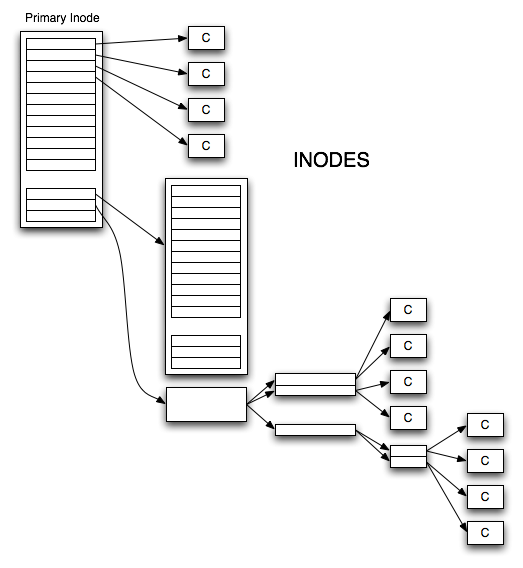
\includegraphics[width=0.6\textwidth]{inodes.png}
\end{figure} 

Cada inodo en el sistema de archivos Minix 1 se identifica por un n\'umero entero positivo entre 1 y 65536. Esto permite por
ejemplo que la organizaci\'on de los directorios siga un esquema de \'arbol (aunque existe la noci\'on de \textit{hard} y \textit{soft}
links en Minix 1, por simplicidad no fueron implementados): Cada inodo de directorio almacena en sus zonas de datos entradas de 32 bytes
que consisten en:

\begin{itemize}
	\item 2 bytes para el numero de inodo correspondiente al hijo.
	\item 30 nombres para el pedazo del nombre del hijo.
\end{itemize}

Por ejemplo, si tuvieramos el archivo \url{/docs/docs/archivo.txt}, \texttt{archivo.txt} ser\'ia el nombre con el que identificar\'iamos en
el inodo del segundo \texttt{docs} al inodo del archivo final. La organizaci\'on es entonces jer\'arquica separada por caracteres de barra
como es usual en los sistemas UNIX.

Por \'ultimo es necesario considerar los archivos correspondientes a drivers. Los drivers en Minix se identifican con dos n\'umeros, el
n\'umero major (que indica el tipo de dispositivo) y el n\'umero minor (que indica una instancia del tipo de dispositivo dado por el otro
n\'umero). Estos dos valores ocupan 1 byte y por lo tanto se almacenan en la primer entrada de zonas del inodo en disco duro. Como esta
entrada tiene tama\~no de 2 bytes, en el byte menos significativo se almacena el major number y en el m\'as significativo el minor number.
 
La distinci\'on entre los distintos tipos de inodo es posible gracias a un flag de identificaci\'on que es parte del inodo. Adem\'as de esto
el inodo en disco mantiene el tama\~no en bytes del archivo.

Finalmente, es necesario mantener ciertos datos sobre la partici\'on utilizada: por ejemplo que inodos est\'an usados o no, la informaci\'on
de cada inodo en una secci\'on encontrable a priori de iniciar la partici\'on, y que zonas en disco est\'an o no libres.

Para esto, toda partici\'on Minix 1 de disco inicia con el bootblock (que contiene la informaci\'on para bootear el sistema operativo en disco
duro, que en nuestro caso no utilizamos puesto que se bootea directamente mediante el diskette) al cual le sigue el denominado \textit{super block}. El super bloque inicia entonces en la segunda zona (Sector n\'umero 3) y contiene la siguiente informaci\'on:

\begin{itemize}
	\item La cantidad de inodos en la partici\'on actual.
	\item La cantidad de zonas de datos disponibles en la partici\'on actual.
	\item Cantidad de bloques correspondientes al mapa de bits de inodos.
	\item Cantidad de bloques correspondientes al mapa de bits de zonas de datos libres.
	\item Zona de inicio de las zonas de datos.
	\item Valor $c$ tal que $2^c$ corresponde al tama\~no en zonas del espacio de datos del disco.
	\item Tama\~no m\'aximo de archivo.
	\item Valor m\'agico que identifica esta partici\'on. En el caso de MINIX 1 este valor es $0x138F$
\end{itemize}

Posteriormente a este super bloque, viene un mapa de bits que codifica que inodos est\'an o no libres, y luego un mapa de bits que codifica
que zonas de datos est\'an o no libres. Ambos mapas de bits son cargados a memoria cuando se inicializa el super bloque en memoria con el
pr\'oposito de utilizar la estructura \texttt{bitset} descripta en la secci\'on~\ref{sec::memory} para administrar estos espacios. Finalmente,
lo que sigue es la zona de inodos: un arreglo contiguo de zonas que almacenan la metainformaci\'on de cada inodo del sistema, o espacio libre
si ese inodo no esta asignado. Puesto que la estructura en disco de un inodo consiste de 32 bytes, la cantidad de estas que entra en 1024 bytes
es entera y nunca cruza un borde de zona. Finalmente, a esto sigue las zonas de datos.

Un esquema de esta organizaci\'on de las primeras zonas del disco se puede ver en la Figura~\ref{fig::superblock}.

\begin{figure}[H]
	\caption{Organizaci\'on de las primeras zonas de una partici\'on de Minix.}
	\label{fig::superblock}
	\centering
	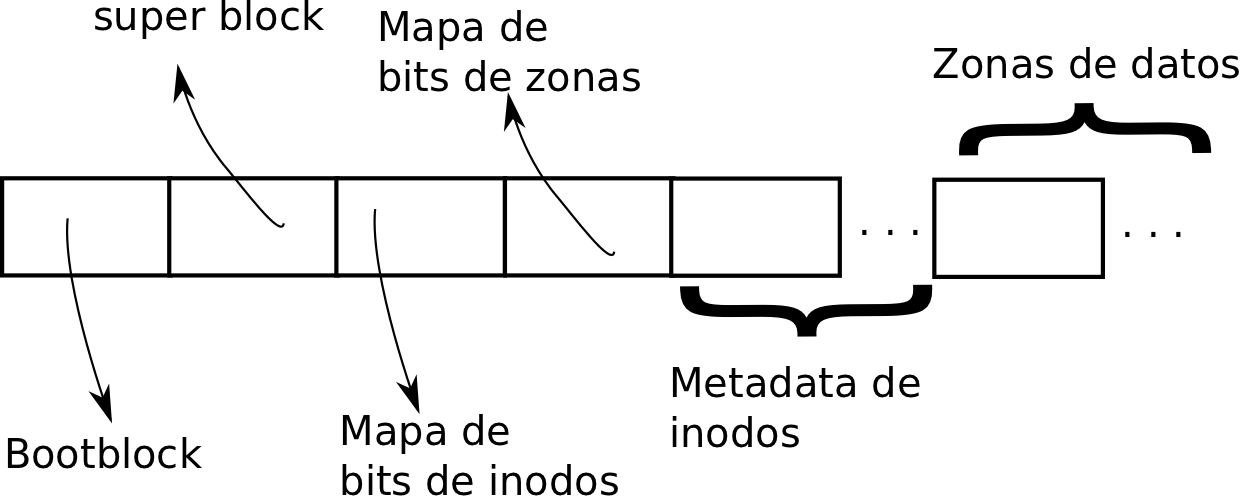
\includegraphics[width=0.6\textwidth]{superblock.png}
\end{figure} 

Otro motivo para utilizar este sistema de archivos es que en el entorno de desarrollo utilizado se disponen de herramientas para crear archivos
que contengan una partici\'on de Minix 1: En particular estamos hablando del comando \texttt{mkfs.minix}. De esta manera, podemos utilizar 
este comando y comandos espec\'ificos para armar im\'agenes de disco para el simulador Bochs para crear una im\'agen de disco con el sistema
de archivos valido y que contenga los valores que deseemos. Esto en particular nos fue muy \'util para resolver problemas no documentados sobre
el sistema de archivos y para adem\'as poder testear el c\'odigo de sistema de archivos por separado al c\'odigo del resto del Sistema Operativo
(mejorando as\'i la modularidad).

Por \'ultimo ahondaremos en dos detalles implementativos: La noci\'on de Virtual Filesystem y la noci\'on de cache de buffers y cache de
inodos.

\subsection{Virtual Filesystem}

La idea de un sistema de archivos virtual es proveer una abstracci\'on por sobre la implementaci\'on particular del sistema de archivos de
manera de poder trabajar de manera general sobre ellos. En nuestro caso, la capa de abstracci\'on se provee mediante las nociones de inodo,
superbloque y file object. Las dos primeras nociones son id\'enticas a las de Minix, con modificaciones que veremos posteriormente. La noci\'on
de file object es la de una instancia de un inodo abierto. Esto sirve por ejemplo para mantener la idea de que estamos leyendo un cierto offset dentro de un inodo y que esto es independiente del inodo en si (que representa un archivo).

La modificaci\'on m\'as importante es que cada uno de estos tres valores provee una abstracci\'on en la forma de una serie de funciones:

\begin{itemize}
	\item El super bloque debe ser capaz de crear, leer de disco, escribir a disco y mantener la consistencia de los inodos en una partici\'on,
	sea esta la que sea. En el caso de Minix por ejemplo se ocupa de mantener la consistencia de los mapas de bits con los inodos en uso y las
	zonas de datos disponibles, y de mantener los metadatos de cada inodo coherentes con su representaci\'on en los caches de memoria RAM.
	\item El inodo debe ser capaz de operar sobre la noci\'on de archivo. Por ejemplo, un inodo de directorio debe proveer funciones para
	buscar el inodo de un subarchivo directo en la jerarqu\'ia, crear subdirectorios y subarchivos, borrar subarchivos, etc. Debe proveer
	adem\'as una abstracci\'on con respecto a que operaciones de acci\'on se pueden realizar sobre \'el: que quiere decir leerlo, escribirlo,
	etc.
	\item Un file object no provee m\'as abstracci\'on que la de ser una instancia de un inodo abierto. Mantiene \'indices dentro del mismo y
	conoce las operaciones que se pueden realizar. Su prop\'osito por sobre todo es ser el objeto interfaz entre los procesos (mediante las
	llamadas a sistema) y el sistema de archivos en si.
\end{itemize}

De esta manera, se tiene una abstracci\'on general que permite por ejemplo el manejo gen\'erico de archivos con un mismo conjunto de llamadas
a sistema (que describiremos en ~\ref{sec::filesystem_syscalls}).

\subsection{Caches de disco y de inodos}

Para evitar posibles problemas de fragmentaci\'on de la heap de kernel, se mantiene un cache de inodos. Esto quiere decir que cuando el sistema operativo
necesita un inodo, busca si uno ya preasignado fue liberado. Si fue liberado, lo utiliza, sino, crea uno nuevo y lo agrega a una lista. Esta
lista es responsabilidad del superbloque de la partici\'on, que la mantiene. De esta manera, no se fragmenta la memoria producto de crear y
liberar muchas veces un inodo, y se mejora la performance y se mantiene una interfaz m\'as simple. Cada inodo lleva para este prop\'osito un
contador de instancias en uso. Si bien el sistema de archivos es \textit{single-threaded} como esta implementado (es decir, se producir\'ian
condiciones de carrera si dos instancias de un proceso por ejemplo actuaran sobre el mismo archivo), este contador de instancias de uso se
podr\'ia utilizar posteriormente para mantener una sola instancia sincronizada en memoria del inodo, manteniendose entonces la consistencia
del sistema de archivos (usandose para ello por ejemplo un esquema de sincronizaci\'on por sem\'aforos).

Para abstraer los accesos a disco, que se hacen por sectores, se implement\'o adem\'as un cache de buffers, muy similar al disponible por
ejemplo en Unix System V (ver~\cite{systemv}). Este cache consiste en una serie de buffers de tama\~no de una zona, linkeados entre si con
una lista enlazada. Cada buffer sabe a que zona y con que desplazamiento esta actuando, y adem\'as sabe si los datos est\'an o no sincronizados
con el disco duro (ya que sabe que operaci\'on se esta realizando sobre \'el). Cuando se desea escribir a disco solamente es necesario indicar
el bloque y offset deseados, y pasar los datos. El cache de buffers se ocupa de buscar el buffer correspondiente si ya esta abierto, y si no
es as\'i se ocupa de encontrar un buffer libre y desalojarlo como corresponda (por ejemplo escribiendolo a disco si estaba sucio). En \'ultima
instancia si no encuentra ninguno lo que hace es agregar un nuevo buffer a la lista enlazada de buffers libres.

Adicionalmente, se mantiene una lista de buffers sucios y a que inodo corresponde cada uno, de manera de poder, en caso de ser pertinente, bajar
los datos a disco de los buffers sucios correspondientes a un inodo (por ejemplo, cuando se realiza un \texttt{close} o un \texttt{flush}).

\subsection{Llamadas de sistema operativo}
\label{sec::filesystem_syscalls}

La interfaz con la que cuentan los procesos es la interfaz de llamadas de sistema de archivos. Estas llamadas son similares a las del estandar
POSIX: Cada proceso guarda una estructura de hasta cierto n\'umero de file objects abiertos. Estos file objects se heredan entre llamadas de
fork y se cierran al terminar el proceso (con excepcion de la entrada y salida estandares que se comparten con el shell como veremos
posteriormente). Al usuario de estas llamadas no se le devuelve un file object directamente sino que se le devuelve un identificador dentro del
arreglo del proceso, mas conocido en la jerga como un \textit{file descriptor}. Este se utiliza para el resto de las llamadas.

A continuaci\'on describimos las llamadas de sistema implementadas.

\begin{itemize}
	\item open: Esta llamada a sistema recibe un directorio y una serie de flags que indican que se desea hacer con el archivo a abrir,
	y el sistema entonces accede al archivo correspondiente, lo prepara para utilizarse, y devuelve un \textit{file descriptor} identificador
	para llamadas posteriores. Si se produjo un error en este proceso, se devuelve el mismo en vez de un descriptor de archivo. Para diferenciar
	identificadores de c\'odigos de error, los c\'odigos de error tienen valores negativos (el mismo sistema se usa para las dem\'as llamadas
	a sistema).

	\item read: Esta llamada a sistema toma un archivo abierto para lectura y lee una cantidad determinada de bytes a un buffer. Para evitar
	indicar el \'indice cada vez, este se mantiene en el \textit{file object} correspondiente, y se actualiza de manera coherente. Si ocurre
	un error en la lectura se retorna un c\'odigo de error. Sino, se retorna la cantidad efectiva de bytes leidos (el sistema de archivos se
	ocupa de evitar que se pase de largo del archivo, lo cual facilita el uso de la interfaz mediante el uso de un buffer).		

	\item write: La llamada es similar a read, pero para escribir a un archivo. A diferencia de read, esta llamada utiliza un flag (que se
	determina a tiempo de apertura del archivo) para indicar si se desea sobreescribir un archivo o agregarle informaci\'on . Tambi\'en esta
	llamada utiliza otro flag para indicar si al intentar escribir un archivo inexistente el mismo debe ser creado (FS\_TRUNC y FS\_CREAT
	especificamente). Tambi\'en se retorna la cantidad de bytes escritos o un error en caso correspondiente.

	\item readdir: Esta llamada es espec\'ifica para directorios y se provee como interfaz por sobre la llamada a read. Lo que hace es leer
	la siguiente entrada de directorio en el archivo a un buffer. Regresa el tama\~no de una de estas entradas o un error como c\'odigo negativo.

	\item close: Indica que el proceso no va a usar m\'as este archivo y que por lo tanto el sistema operativo debe liberar los recursos
	asignados a este.
\end{itemize}

Para m\'as informaci\'on puede consultarse~\cite{minixfs}. Dada la falta de documentaci\'on del sistema de archivos Minix, dado que el autor no pudo conseguir una copia de \textit{Operating Systems Design and Implementation} correspondiente a las primeras ediciones, parte de los detalles
fueron descubiertos por el mismo autor mediante el ex\'amen minuscioso de im\'agenes de disco construidas con el comando \texttt{mkfs.minix} y examinadas byte por byte con el uso del comando \texttt{hdd}.


\section{Posibilidades de expansi\'on}
\label{sec::expansion}

\epigraph{Regression testing? What's that? If it compiles, it is good; if it boots up, it is perfect.}{Linus Torvalds}

Considerando las limitaciones se\~naladas en este trabajo, proponemos
que siguientes trabajos podr\'ian expandir lo realizado en este en las
siguientes \'areas:

\begin{itemize}
	\item Quitar la no preemptabilidad del kernel. Esto requiere la
	implementaci\'on de un sistema de exclusi\'on m\'utua para proteger
	las \'areas compartidas del sistema operativo de acceso concurrente
	(como por ejemplo el asignador de memoria o la lista de procesos).
	Adicionalmente, requiere tomar una soluci\'on con respecto al problema
	de PC Losering, es decir como debe manejar el Sistema Operativo una
	se\~nal o interrupcci\'on cuando esta realizando el servicio de una
	llamada de Sistema. Posibles soluciones a este problema var\'ia y
	recomendamos \url{http://www.jwz.org/doc/worse-is-better.html} donde se
	introduce y discute la tem\'atica.
	\item Implementar m\'as caracter\'isticas de consola, como por ejemplo
	redirecci\'on de entrada salida y uni\'on de comandos mediante \texttt{pipes}
	cl\'asicos de Unix. Tambi\'en se har\'ia necesario implementar \textit{job control
	groups} para dar una interfaz esperable sobre la entrada para que los procesos
	puedan leer de entrada salida estandar.
	\item Agregar soporte de concurrencia al sistema de archivos, mediante un sistema
	de exclusi\'on m\'utua. Esto requerir\'ia por ejemplo implementar sem\'aforos y
	agregarselos a los inodos y al cach\'e de buffers (usando patrones como por ejemplo
	productor consumidor, para m\'as informaci\'on v\'ease~\cite{semaphores}). Esto se
	hace imperante si se desea adem\'as agregar acceso a disco no bloqueante o mediante
	el uso de DMA (Direct Memory Access).
	\item Agregar caracter\'isticas al sistema de archivos, como por ejemplo particiones
	multiples, \textit{symlinks}, filesystems multiples (usando la capa de Virtual Filesystem
	implementada actualmente), soporte para filesystems en block devices no basados en disco
	\item Implementar un driver en modo usuario de VGA o VESA para permitir mayores
	resoluciones. Tambi\'en podr\'ia implementarse un driver de sonido para placas Sound Blaster.
	\item Agregar una etapa de detecci\'on de hardware y modificar el driver de disco duro para
	que utilice PCI Busmastering DMA y permita multiples discos duros ATA (no solo un master).
	\item Implementar m\'as programas a nivel de usuario.
	\item Implementar librer\'ias compartidas y agregar soporte para linkeo din\'amico.
	\item Implementar un esquema de \texttt{swapping} de p\'aginas a disco.
	\item Optimizar los algoritmos: Un lugar posible de optimizaci\'on es reducir la
	cantidad de b\'usquedas secuenciales mediante el uso de tablas de Hashing o diccionarios
	similares.
	\item Implementar m\'as llamadas a sistema y posiblemente convertir las existentes para que
	sean POSIX compatibles.
	\item Usar esquemas de paginaci\'on m\'as modernos en caso de detecci\'on para soportar m\'as
	de 4 Gb de memoria (por ejemplo PAE Paging).
	\item Portear el c\'odigo a IA 64.
\end{itemize}

Todos estas posibles mejoras se han tenido en cuenta en el dise\~no actual (si bien no est\'an implementadas)
de manera que no debiera ser necesario un redise\~no completo para implementarlas (aunque si posiblemente se
debe tener cuidado en especial con las que involucran acceso concurrente). Dejamos estas \'areas como posibilidades
de expansi\'on.

\section{Conclusi\'on}

El Sistema Operativo implementado, si bien es crudo en funcionalidad y tiene varias \'areas posibles de optimizaci\'on,
sirvi\'o para organizar y experimentar con distintos aspectos del diseño de un sistema de estas caracter\'isticas, en especial
que m\'odulos es necesario tener y como se pueden abstraer detalles de la arquitectura pero usarlos de manera de implementar
funcionalidad. El trabajo tambi\'en sirve como base y punto de expansi\'on para trabajar con otros conceptos de Sistemas Operativos
y hace uso de la arquitectura IA 32 de manera de mostrar como se pueden emplear los recursos que esta provee.

\section{Agradecimientos}

Se agradece a Christian Heitman por sus \'utiles links y comentarios, sin los cuales este trabajo hubiese probablemente sido inatacable,
y a Manuel Ferreria por su ayuda en la verificaci\'on de la im\'agen entregable.


\addcontentsline{toc}{section}{Referencias}
\begin{thebibliography}{9}

\bibitem{ataspec}
	Especificaci\'on ATA, disponible en \url{http://hddguru.com/content/en/documentation} y
	c\'odigo ejemplo en \url{http://www.ata-atapi.com/}
\bibitem{jamesmolloy}
	James Molloy,
	\textit{Roll your own toy UNIX-clone OS},
	tutorial disponible en \url{http://www.jamesmolloy.co.uk/tutorial_html/index.html}

\bibitem{systemv}
	Maurice Bach,
	\textit{The Design of the Unix Operating System}
	Prentice Hall Software Series, 
	1986	

\bibitem{intel2}
	Intel 64 and IA-32 Architectures
	Software Developer’s Manual,
	\textit{Volume 2 (2A \& 2B): Instruction Set Reference, A-Z}

\bibitem{intel3}
	Intel 64 and IA-32 Architectures
	Software Developer’s Manual,
	\textit{Volume 3A: System Programming Guide, Part 1}

\bibitem{linux}
	Bovet, Daniel P. y Cesati, Marco
	\textit{Understanding the Linux Kernel},
	O'Reilly Media, 2000
	
\bibitem{kr}
	Kernighan, Brian y Ritchie, Dennis
	\textit{The C Programming Language, 2nd Edition},
	Pearson Education, 1991 

\bibitem{abi}
	System V ABI Especification, \url{http://www.sco.com/developers/devspecs/gabi41.pdf}

\bibitem{osdev}
	Wiki de OSDEV, \url{wiki.osdev.org}, en particular los art\'iculos:
	\begin{itemize}
		\item ATA PIO
		\item CMOS clock
		\item ELF
		\item Bare Bones Tutorial
	\end{itemize}

\bibitem{osdever}
	Bona Fide OS Developer Tutorials, en particular:
	\begin{itemize}
		\item Memory Management 1 y 2 por Tim Robbins.
		\item LBA HDD Access via PIO por Dragoniz3r.
		\item Bran's Kernel Development Tutorial por Brandon F.
		\item Using GRUB por Chris Giese.
	\end{itemize}

\bibitem{gnugrub}
	Especificaci\'on Multiboot por la GNU Free Software Foundation,
	\url{www.gnu.org/software/grub/manual/multiboot/multiboot.html}

\bibitem{semaphores}
	Downey, Allen B.
	\textit{The Little Book of Semaphores},
	Green Tea Press, 2008,
	\url{http://www.greenteapress.com/semaphores/downey08semaphores.pdf}

\bibitem{minixfs}
	Heavner, Scott D.
	\textit{Introduction to the Minix File System},
	\url{http://ohm.hgesser.de/sp-ss2012/Intro-MinixFS.pdf}

\end{thebibliography}


\end{document}
